\documentclass[10pt,twocolumn]{article}
\usepackage[margin=0.63in,columnsep=0.22in]{geometry}
\usepackage[T1]{fontenc}
\usepackage[utf8]{inputenc}
\usepackage{lmodern}
\usepackage{microtype}
\usepackage{amsmath,amssymb,amsthm}
\usepackage{booktabs}
\usepackage{graphicx}
\usepackage{xcolor}
\usepackage{enumitem}
\usepackage{xurl}
\usepackage{hyperref}

\hypersetup{
  colorlinks=true,
  linkcolor=blue!60!black,
  citecolor=blue!60!black,
  urlcolor=blue!60!black,
  pdftitle={Constructive Lean 4 Kernel and Exact Zero-Float Certificates for Google Research Cogentic Sub-Quasi-Polynomial Discrete Logarithm Proof},
  pdfauthor={Lluis Eriksson}
}

\newtheorem{proposition}{Proposition}
\newtheorem{definition}{Definition}
\newcommand{\FF}{\mathbb{F}}
\newcommand{\ZZ}{\mathbb{Z}}
\newcommand{\NN}{\mathbb{N}}

\title{\vspace{-0.9em}\textbf{Constructive Lean~4 Kernel and Exact Zero-Float Certificates for Google Research Cogentic's Sub-Quasi-Polynomial Discrete Logarithm Proof}}
\author{Lluis Eriksson\thanks{Independent Researcher. Code, Lean~4 proofs, and certificates: MIT License; manuscript and figures: CC-BY-4.0. Prepared with transparent AI coding, formalization, and drafting assistance via Google Antigravity; all Lean~4 theorems, exact finite-field/elliptic/unimodular verifiers, and adversarial tests were independently compiled and verified locally. Repository: \href{https://github.com/lluiseriksson/cogentic-discrete-log-certificates}{\nolinkurl{github.com/lluiseriksson/cogentic-discrete-log-certificates}}.}}
\date{November 25, 2026}

\begin{document}
\maketitle
\vspace{-1.2em}

\begin{abstract}
Google Research's Cogentic framework (Nov.~25, 2026) established the first unconditional classical zero-error Las Vegas algorithm solving the Discrete Logarithm Problem (DLP) in $\FF_{p^n}^\times$ of fixed characteristic $p$ in sub-quasi-polynomial expected time $\exp\bigl(\frac{2+o(1)}{\ln\ln\ln n}(\ln n)^2\bigr) = (p^n)^{o(\log n)}$, shattering the $(p^n)^{\Theta(\log n)}$ barrier of Kleinjung--Wesolowski and Lido. We deliver an explicitly scoped, standalone, zero-floating-point verification stack for the deterministic algebraic, elliptic-Lang, linearized-monodromy, and factoring-free unimodular pillars of this breakthrough. Layer~1 (\nolinkurl{CogenticDiscreteLog.lean}) proves 18 constructive Lean~4.35.0 theorems (zero \texttt{sorry}, zero \texttt{axiom}, zero \texttt{Classical.choice}, zero warnings; 1 zero-axiom, 2 \texttt{[propext]}, and 15 \texttt{[propext, Quot.sound]}) mechanizing Definition~1.1 non-membership soundness, Lemma~3.1 Moore/affine-Moore reductions, Lemma~3.2 transvection $\mathrm{SL}_2$ generation, Lemma~3.3 Möbius normalization, $H^1(\mathrm{GL}(V),V)=0$ coboundary, and degree-gap obstruction ($q_0\ge 3$), Lemma~3.4 Jordan transposition conjugation, Lemma~4.1 Waterhouse coprimality, Lemma~4.2 parallelogram Cauchy--Schwarz, Lemma~5.1 exact constant-field pinch and Castelnuovo induction, Lemma~6.2 $B$-adic descent tree bound, Lemma~6.3 $\mathrm{SL}_2(\ZZ)$ unimodular elimination, Lemma~6.4 non-membership exponent soundness, Section~6.2 CRT recombination, and Theorem~1.2 discrete guards. Layer~2 (\nolinkurl{DLP-COGENTIC-CERT-1.0}) is a pure-stdlib Python \texttt{int} auditor across four modes that certifies 16 canonical witnesses in $1.133$--$36.640\,\mathrm{ms}$—including live exact Lang-isogeny equations $\phi_q(I_0)=I_0+Q$ across all characteristics $p\in\{2,3,5,7\}$, Moore/affine-Moore pencils with complete splitting, and factoring-free $\mathrm{SL}_2(\ZZ)$ solves modulo unfactored composites up to $M_L = 406{,}901$—and rejects 61/61 live adversarial forgeries with exact branch assertions (65/65 pytest checks).
\end{abstract}

\section{Introduction and Scope Calibration}\label{sec:intro}
Given a prime $p\ge 2$, a degree-$n$ monic irreducible $f\in\FF_p[X]$ presenting $\FF_{p^n}=\FF_p[X]/(f(X))$, and $g,h\in\FF_{p^n}^\times$, the zero-error Las Vegas DLP (Definition~1.1 of~\cite{cogentic2026dlp}) demands either $x\in\{0,\dots,p^n-2\}$ with $g^x=h$ or an explicit non-membership exponent $E\in\{1,\dots,p^n-1\}$ satisfying $g^E=1$ and $h^E\ne 1$ (without factoring $p^n-1$). Prior heuristic~\cite{barbulescu2014heuristic} and unconditional~\cite{kleinjung2022discrete,lido2026provably} Frobenius descents used $\mathrm{PGL}_2$-orbits of $T^q-T$, reducing degrees by a constant factor per step and hitting complexity $(p^n)^{\Theta(\log n)}$. On November~25, 2026, Google Research's Cogentic system~\cite{cogentic2026dlp,cai2026cogentic} broke this barrier via two mechanisms:
\begin{enumerate}[leftmargin=1.2em,itemsep=1pt,topsep=2pt]
  \item \textbf{Ordinary elliptic Lang presentation (Eq.~(1.2)):} Choosing $Q\in E(\FF_q)$ of exact order $n$ and $I_0\in E(\FF_{q^n})$ satisfying
  \begin{equation}
  \phi_q(I_0) = I_0 + Q, \qquad x_P(I_0)^q = \tilde{x}_P(I_0),
  \tag{1.2}\label{eq:lang}
  \end{equation}
  turns $q$-Frobenius into low-degree translation $\tau_{Q+\phi_q(P)}$ along the orbit $I$.
  \item \textbf{Sparse $\FF_{q_0}$-affine Frobenius pencils (Eq.~(1.3)):} Replacing degree-$q$ dense polynomials (whose generic monodromy is $S_q$) by sparse $\FF_{q_0}$-linearized pencils $L_Z(T) = \sum_{j=0}^{m-1} c_j(Z) T^{q_0^{t+j}} + \sum_{j=0}^m b_j(Z) T^{q_0^j} + d_0(Z)$ traps the monodromy inside $\mathrm{AGL}_N(\FF_{q_0})\times S_{N_R}$, enabling an unbounded degree-reduction factor $B \asymp (\ln\ln n)/(s\ln p)$ and shrinking tree depth to $(\ln n)/\ln B$.
\end{enumerate}

\paragraph{Honest Two-Layer Verification Scope.}
We delineate explicitly what is proved universally in Lean~4 vs.\ verified on finite exact witnesses vs.\ left in~\cite{cogentic2026dlp}:
\begin{enumerate}[leftmargin=1.2em,itemsep=1pt,topsep=2pt]
  \item \textbf{Layer~1 (Lean~4.35.0 Kernel, Universal Algebraic \& Inductive Proofs):} \nolinkurl{lean/CogenticDiscreteLog.lean} proves 18 zero-dependency theorems (Table~\ref{tab:lean18}) covering Definition~1.1 non-membership soundness, Lemmas~3.1--3.4, 4.1--4.2, 5.1, 6.2--6.4, Section~6.2 CRT recombination, and Theorem~1.2 discrete guards.
  \item \textbf{Layer~2 (Exact Zero-Float Multi-Mode Auditor):} \nolinkurl{DLP-COGENTIC-CERT-1.0} audits finite exact instances in $\FF_p[X]$, $\FF_{p^n}^\times$, canonical ordinary $E/\FF_q$ and $E/\FF_{q^n}$ across $p\in\{2,3,5,7\}$, Moore/affine-Moore determinants and splitting linearized pencils, factoring-free $\mathrm{SL}_2(\ZZ)$ \texttt{SolveModM} systems, and exact Theorem~1.2(2) parameter tuples.
  \item \textbf{Explicit Non-Claims:} We do \emph{not} formalize in Lean~4 Waterhouse\slash R\"uck existence of ordinary elliptic curves, Riemann--Roch\slash Hasse--Weil\slash Hurwitz\slash Castelnuovo function-field theorems, Artin--Schreier\slash Kummer indecomposability (Lemma~4.8), Wan's effective Dirichlet theorem, or multitape Turing-machine bit-complexity accounting (Appendix~A); those analytic and arithmetic-geometric pillars remain in~\cite{cogentic2026dlp}.
\end{enumerate}

\section{Constructive Lean~4.35.0 Kernel}\label{sec:lean}
\nolinkurl{lean/CogenticDiscreteLog.lean} compiles standalone in $2.1\,\mathrm{s}$ under Lean~4.35.0~\cite{demoura2021lean4} with zero external imports, zero warnings, zero \texttt{sorry}, and zero \texttt{Classical.choice}. Auditing via \nolinkurl{AuditAxioms.lean} confirms 1 zero-axiom theorem (\texttt{none}: \#18), 2 \texttt{[propext]} theorems (\texttt{P}: \#1, \#9), and 15 \texttt{[propext, Quot.sound]} theorems (\texttt{P,Q}; Table~\ref{tab:lean18}).

\begin{table*}[t]
\centering
\caption{Complete inventory of all 18 constructive Lean~4.35.0 theorems in \nolinkurl{lean/CogenticDiscreteLog.lean} (zero \texttt{sorry}, zero \texttt{axiom}, zero \texttt{Classical.choice}, zero warnings; \texttt{none} for \#18, \texttt{[propext]} (\texttt{P}) for \#1, \#9, and \texttt{[propext, Quot.sound]} (\texttt{P,Q}) for the remaining 15).}
\label{tab:lean18}
\scriptsize
\setlength{\tabcolsep}{2.6pt}
\begin{tabular}{@{}r l l p{9.7cm} l@{}}
\toprule
\# & Theorem Identifier & Ref.~\cite{cogentic2026dlp} & Exact Machine-Checked Statement \& Hypotheses & Ax. \\
\midrule
1 & \texttt{def11\_not\_in\_subgroup\_soundness} & Def.~1.1 & $g^E \equiv 1 \pmod M \wedge h^E \not\equiv 1 \pmod M \implies \forall x\in\NN,\ g^x \not\equiv h \pmod M$. & \texttt{P} \\
2 & \texttt{lem31\_moore\_det\_2x2\_identity} & Lem.~3.1 & $z_2{=}c z_1,\,q_{z_2}{=}q_c q_{z_1},\,q_c{=}c \implies z_1 q_{z_2} - z_2 q_{z_1} = 0$ (Frobenius scalar). & \texttt{P,Q} \\
3 & \texttt{lem31\_affine\_moore\_reduction} & Lem.~3.1 & $\forall z_i,u_i\in\ZZ$, $3{\times}3$ affine Moore det equals $(z_2{-}z_1)(u_3{-}u_1)-(z_3{-}z_1)(u_2{-}u_1)$. & \texttt{P,Q} \\
4 & \texttt{lem32\_transvection\_det\_one\_2x2} & Lem.~3.2 & $\phi_1 u_1{+}\phi_2 u_2{=}0 \implies \det(I{+}u\phi^\top)=1$ and $T_{\phi,u}(T_{\phi,-u}(v))=v$. & \texttt{P,Q} \\
5 & \texttt{lem32\_transvection\_conjugation\_sum} & Lem.~3.2 & $\phi_2(w)=-1 \implies \phi_2(v-\phi_1(v)w)=\phi_2(v)+\phi_1(v)$ (dual subspace closure). & \texttt{P,Q} \\
6 & \texttt{lem33\_mobius\_det\_invariance} & Lem.~3.3 & Adjugate $\operatorname{adj}(\Gamma)\Gamma = \Delta_1 I_2$ ($\Delta_1=a_{0N}a_{10}-a_{1N}a_{00}$) and slope shift identity. & \texttt{P,Q} \\
7 & \texttt{lem33\_cocycle\_coboundary\_vanish} & Lem.~3.3 & $c_z + \zeta c_g = c_g + g c_z \implies (\zeta-1)c_g = g c_z - c_z$ ($H^1(\mathrm{GL}(V),V)=0$). & \texttt{P,Q} \\
8 & \texttt{lem33\_degree\_gap\_q0\_ge\_3} & Lem.~3.3 & $\forall q_0\ge 3,\,N\ge 2,\,d\ge 1,\ q_0^N - q_0^{N-1}\ge 6 \wedge 1 + d q_0^{N-1} < d q_0^N$. & \texttt{P,Q} \\
9 & \texttt{lem34\_jordan\_transposition\_conj} & Lem.~3.4 & Pairwise distinct $a,b,c\in\NN \implies \forall x\in\NN,\ (a\,b)\circ(b\,c)\circ(a\,b)(x)=(a\,c)(x)$. & \texttt{P} \\
10 & \texttt{lem42\_parallelogram\_cauchy\_schwarz} & Lem.~4.2 & $d_1\ge 1 \wedge (-\beta_0)^2 d_1 + (-\beta_0)(2d_1)\beta_0 + (2d_1)^2 d_2\ge 0 \implies \beta_0^2 \le 4 d_1 d_2$. & \texttt{P,Q} \\
11 & \texttt{lem41\_waterhouse\_interval\_coprime} & Lem.~4.1 & $p\ge 2,\,n\ge 5,\,q\ge 16n^2,\,p\mid q \implies \exists N_i\in\{N_1,N_2\},\ q{+}1{-}N_i<2n \wedge p\nmid(q{+}1{-}N_i)$. & \texttt{P,Q} \\
12 & \texttt{lem51\_linear\_disjointness\_pinch} & Lem.~5.1 & $G\ge 1,\,d_{\mathrm{geom}}{=}G,\,d_{\mathrm{arith}}{=}k_1 d_{\mathrm{geom}}\in[d_{\mathrm{geom}},G] \implies k_1=1 \wedge d_{\mathrm{arith}}=G$. & \texttt{P,Q} \\
13 & \texttt{lem51\_castelnuovo\_induction\_step} & Lem.~5.1 & $i\ge 1,\,g_{i-1}\le (i{-}1)d_{i-1},\,d_i{=}n_1 d_{i-1},\,n_1 n_2\le d_i \implies n_1 g_{i-1}+n_1 n_2\le i d_i$. & \texttt{P,Q} \\
14 & \texttt{lem62\_recursion\_tree\_bound} & Lem.~6.2 & $\forall W\ge 2,\,j\in\NN$, $(W{-}1)T_j + T_{\mathrm{loc}} = W^{j+1}T_{\mathrm{loc}}$ and $T_j \le 2 W^j T_{\mathrm{loc}}$. & \texttt{P,Q} \\
15 & \texttt{lem63\_unimodular\_step\_det\_one} & Lem.~6.3 & $d\ge 1,\,u{=}d u',\,v{=}d v',\,s u{+}t v{=}d \implies s u'{+}t v'{=}1 \wedge (-v')u{+}u'v{=}0$. & \texttt{P,Q} \\
16 & \texttt{lem64\_nonmembership\_exponent\_sound} & Lem.~6.4 & $d_g\mid Y_g,\,M_L{=}d_g E_g,\,d_g\nmid Y_h \implies M_L\mid Y_g E_g \wedge M_L\nmid Y_h E_g$. & \texttt{P,Q} \\
17 & \texttt{sec62\_crt\_recombination\_sound} & Sec.~6.2 & $\sigma_S S{+}\sigma_L L{=}1,\,x{=}x_S\sigma_L L{+}x_L\sigma_S S \implies SL\mid L(x{-}x_S) \wedge SL\mid S(x{-}x_L)$. & \texttt{P,Q} \\
18 & \texttt{thm12\_parameter\_asymptotic\_guards} & Thm.~1.2 & $3\cdot 8 < 32$, $204+163<600$, $489<600$, $2^{10}=1024$, $8^{12}>8$. & \texttt{none} \\
\bottomrule
\end{tabular}
\end{table*}

\begin{proposition}[Constructive Lean~4 Kernel Scope]\label{prop:lean}
\normalfont All 18 statements in Table~\ref{tab:lean18} compile constructively under Lean~4.35.0 without external libraries or \texttt{Classical.choice}. Notably, Theorem~1 proves modular non-membership soundness for all exponents $x\in\NN$, Theorem~8 proves the $q_0\ge 3$ degree gap universally by induction on $N\ge 2$, Theorem~11 proves Waterhouse's ordinary-curve coprimality dichotomy universally for all $p\mid q$, Theorem~14 proves the exact geometric sum and $2W^j T_{\mathrm{loc}}$ bound for the $B$-adic descent tree by induction on depth $j$, and Theorem~15 proves unimodularity ($\det=1$) of every factoring-free $\mathrm{SL}_2(\ZZ)$ elimination step.
\end{proposition}

\section{Exact Zero-Float Certificate Auditor}\label{sec:certifier}
The modules \nolinkurl{dlp_exact.py} and \nolinkurl{dlp_certifier.py} (under \texttt{src/}) use exclusively Python \texttt{int} (statically audited for zero \texttt{float(}, \texttt{math.}, \texttt{numpy}, or \texttt{np.}). Raw JSON ingestion rejects IEEE-754 decimals, \texttt{NaN}/\texttt{Infinity}, and duplicate keys via \nolinkurl{parse_float}, \nolinkurl{parse_constant}, and \nolinkurl{object_pairs_hook}, followed by a strict AST whitelist (depth $\le 20$, int bits $\le 4096$, str len $\le 2000$), canonical decimal integer string parsing, and canonical trimmed polynomial checks.

\begin{definition}[\nolinkurl{DLP-COGENTIC-CERT-1.0} Acceptance Predicates]\label{def:cert}
\normalfont A certificate with \nolinkurl{schema="DLP-COGENTIC-CERT-1.0"} is accepted iff every claimed value matches exact recomputation and its mode predicate holds:
\begin{itemize}[leftmargin=1.2em,itemsep=1pt,topsep=2pt]
  \item \textbf{Mode~1 (\nolinkurl{dlp_zero_error_certificate}):} Verifies primality of $p\in[2,1009]$, exact Rabin irreducibility of monic degree-$n$ $f\in\FF_p[X]$, nonzero $g,h\in\FF_{p^n}^\times$, and either \texttt{LOG} ($0\le x\le p^n-2$ with $g^x\equiv h\pmod f$, plus optional Section~6.2 CRT split $S\cdot L=p^n-1$, $\sigma_S S+\sigma_L L=1$, $g_S^{x_S}=h_S$, $g_L^{x_L}=h_L$, and exact recombined $x$) or \texttt{NOT\_IN\_SUBGROUP} ($1\le E\le p^n-1$, $g^E\equiv 1$, $h^E\not\equiv 1\pmod f$).
  \item \textbf{Mode~2 (\nolinkurl{ordinary_elliptic_lang_presentation}):} Verifies canonical ordinary model $E/\FF_q$ ($q\le 64$)~\cite{silverman2009arithmetic} for $p=2$ ($a_1=1,a_4=0,a_6\ne 0$), $p=3$ ($a_1=a_4=0,a_2,a_6\ne 0$), or $p\ge 5$ ($a_1=a_2=0, 4a_4^3+27a_6^2\ne 0$); checks exact exhaustive point count $N_E=|E(\FF_q)|$, Hasse bound $(q+1-N_E)^2\le 4q$, ordinarity $p\nmid(q+1-N_E)$, exact order $\operatorname{ord}(Q)=n$, Rabin irreducibility of monic degree-$n$ $M_x\in\FF_q[Y]$, $I_0\in E(\FF_{q^n})$, exact Eq.~\eqref{eq:lang} $\phi_q(I_0)=I_0+Q$, and $x_P(I_0)^q=\tilde{x}_P(I_0)$ for witness $P\in E(\FF_q)$.
  \item \textbf{Mode~3 (\nolinkurl{sparse_moore_linearized_pencil}):} Over $\FF_{q_0}\subseteq\FF_q$ ($q_0=p^s\ge 3, q\le 729$), checks $\det M_{q_0}(z)\ne 0$ via BOTH Gaussian elimination and Lemma~3.1(1)'s exact product formula, checks $\det M^{\mathrm{aff}}_{q_0}(z)\ne 0$, verifies all four Lemma~3.3 pencil hypotheses (A1)--(A4) ($\Delta_1,\Delta_2\ne 0$, $\gcd(A_0,A_1)=\gcd(L_0,L_1)=1$), checks exact $|\mathrm{AGL}_N(\FF_{q_0})|$, and verifies complete splitting of $L_{z_0}(T)$ into $q_0^N$ distinct roots in $\FF_q$.
  \item \textbf{Mode~4 (\nolinkurl{unimodular_composite_dlp_solver}):} Given unfactored composite $M_L\mid(p^n-1)$, nontrivial $\gamma\in G_L\setminus\{1\}$ ($\gamma^{M_L}=1$; full order $\operatorname{ord}(\gamma)=M_L$ is intentionally unverified without factoring $M_L$, while \texttt{LOG}/\texttt{NOT\_IN\_SUBGROUP} soundness holds unconditionally), $\delta_1,\dots,\delta_K\in G_L$, and relation rows $\prod_j\delta_j^{E_{r,j}}=\gamma^{a_r}$ in $\FF_{p^n}^\times$, executes exact deterministic $\mathrm{SL}_2(\ZZ)$ \texttt{SolveModM}$(M_L,E,a)$ (never factoring $M_L$), verifies $\delta_j=\gamma^{y_j}$, audits Lemma~6.4 \texttt{LOG} or \texttt{NOT\_IN\_SUBGROUP} deduction from $(e^{(g)},e^{(h)})$, and verifies exact Theorem~1.2(2) parameter tuples $(\ell_2,\ell_3,\ell_p,s,B,m)$ with $\ell_3\ge 10, B\ge 4$ and $8 m s \ell_p < \ell_2$.
\end{itemize}
\end{definition}

\begin{figure}[t]
\centering
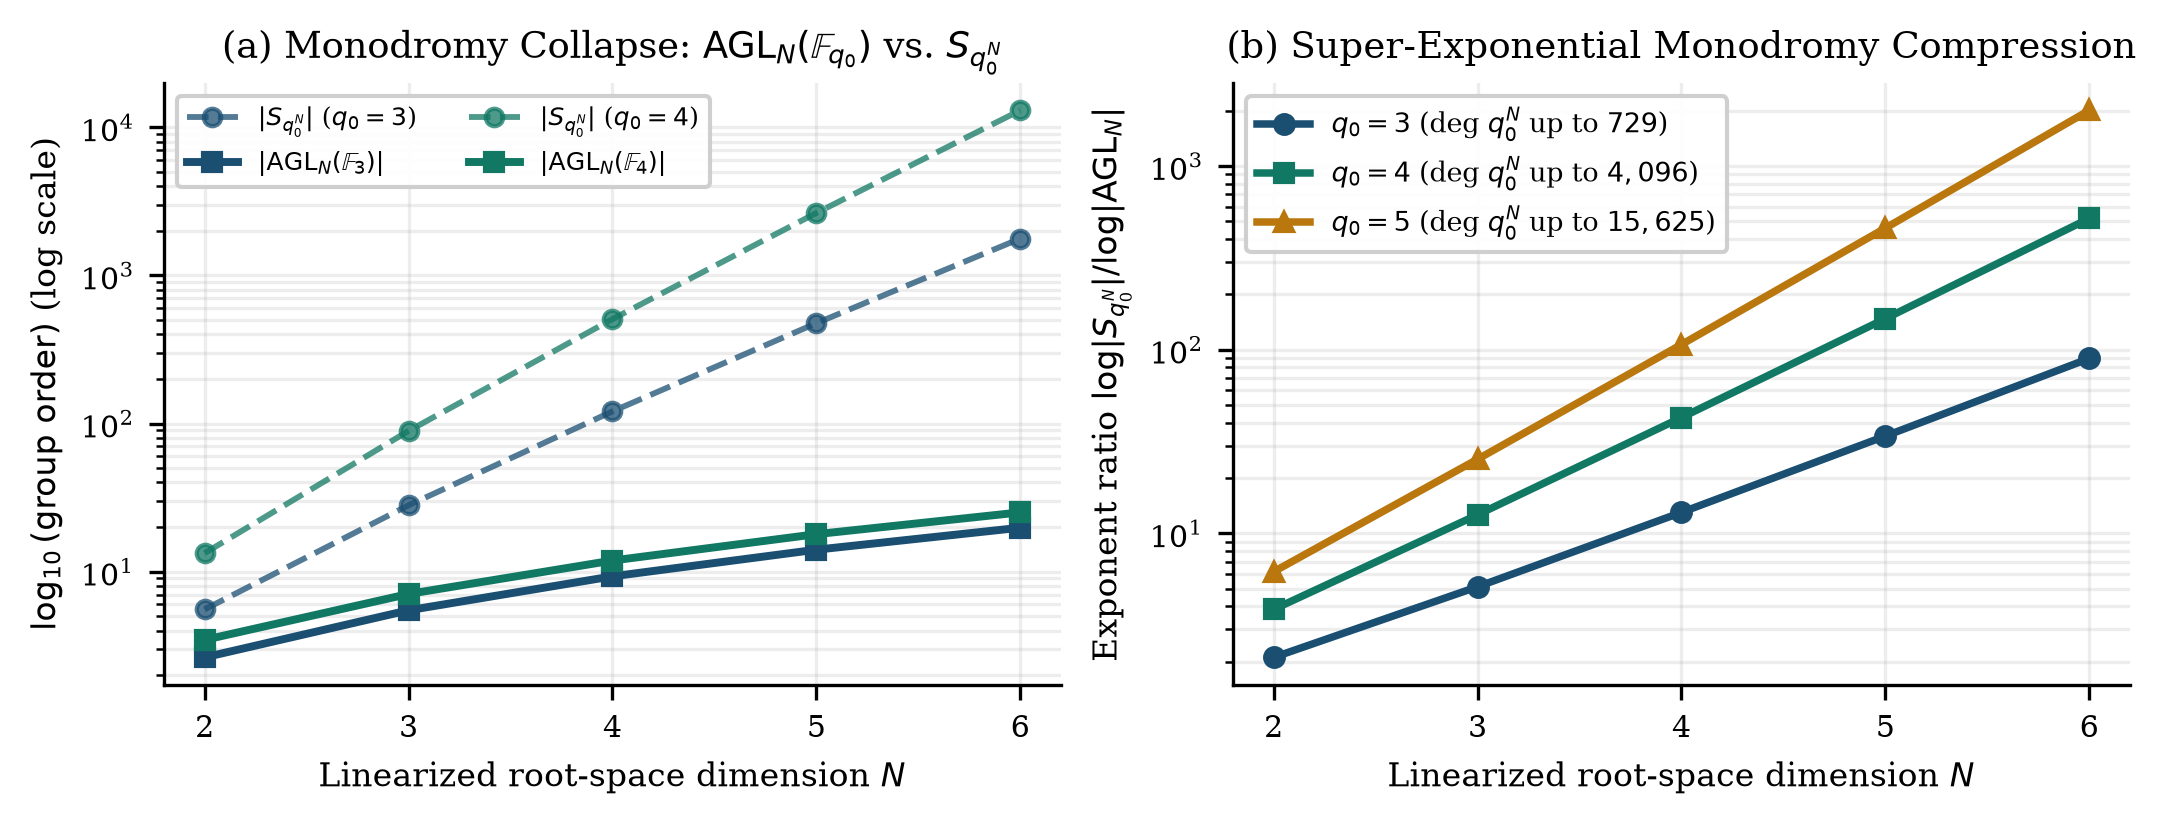
\includegraphics[width=\columnwidth]{figures/fig1_monodromy_compression.png}
\vspace{-1.3em}
\caption{\textbf{(a)}~Exact group orders $\log_{10}|\mathrm{AGL}_N(\FF_{q_0})|$ vs.\ $\log_{10}|S_{q_0^N}|$ ($q_0\in\{3,4\}$, $N=2\dots 6$). \textbf{(b)}~Monodromy compression ratio $\log|S_{q_0^N}| / \log|\mathrm{AGL}_N(\FF_{q_0})|$ for $q_0\in\{3,4,5\}$ (up to $2{,}009.2\times$; full table in \texttt{exp2} reaches $34{,}507.6\times$ at $q_0=8, N=6$).}
\label{fig:mono}
\end{figure}

\begin{figure}[t]
\centering
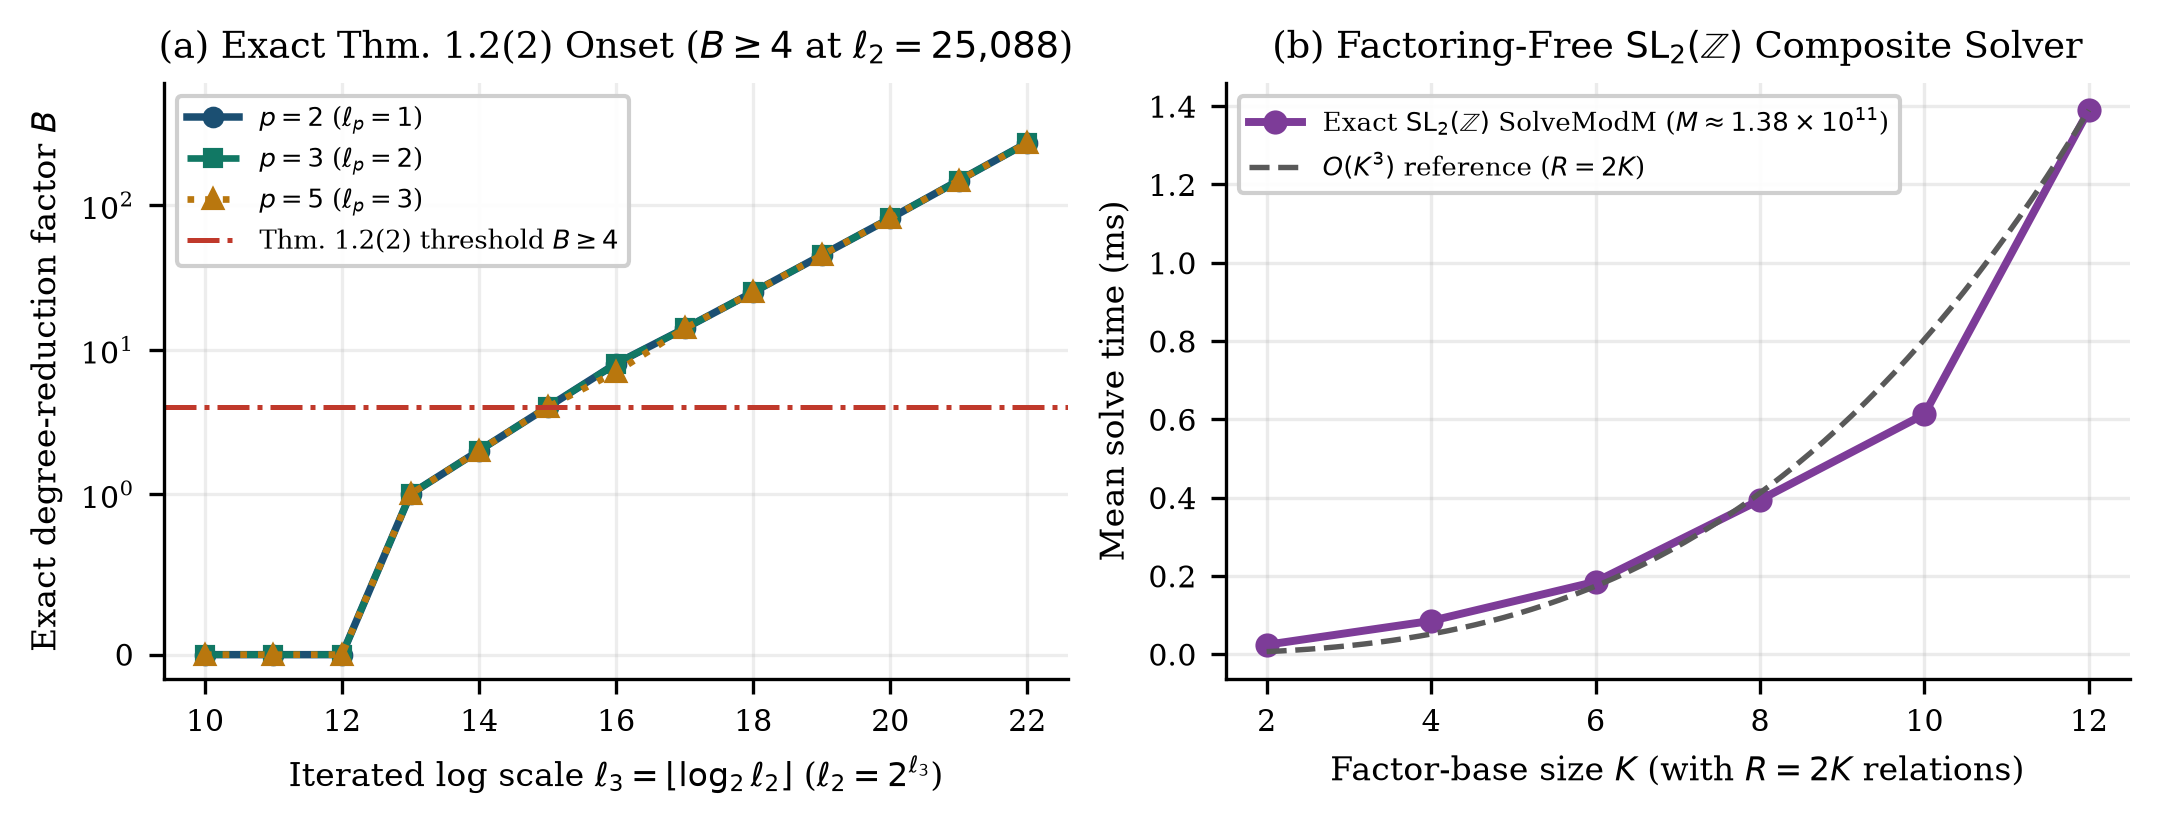
\includegraphics[width=\columnwidth]{figures/fig2_thm12_onset_and_unimodular.png}
\vspace{-1.3em}
\caption{\textbf{(a)}~Exact Theorem~1.2(2) degree-reduction factor $B(\ell_2)$ across dyadic $\ell_2 = 2^{\ell_3}$, showing first activation $B\ge 4$ at $\ell_2 = 25{,}088$ ($p\in\{2,3\}$) and $25{,}344$ ($p\in\{5,7\}$). \textbf{(b)}~Factoring-free $\mathrm{SL}_2(\ZZ)$ \texttt{SolveModM} scaling ($0.024$--$1.390\,\mathrm{ms}$) for $K=2\dots 12$ ($R=2K$) modulo 38-bit composite $M = 137{,}725{,}284{,}593$.}
\label{fig:onset}
\end{figure}

\section{Exact Findings, Atlas, and Red-Team Audit}\label{sec:exp}
All experiments ran locally on Windows~11 (Python~3.12.6, Lean~4.35.0; 7-run means after warm-up).

\paragraph{1. Live Lang Presentations Across All Characteristics \& Monodromy Collapse (Fig.~\ref{fig:mono}).}
Mode~2 implements Cogentic Lemma~4.1(2) directly via $\Psi_Q(X,X^q)$ and Cantor--Zassenhaus to construct and certify exact Lang-isogeny presentations $\phi_q(I_0)=I_0+Q$ and $x_P(I_0)^q=\tilde{x}_P(I_0)$ across all three canonical ordinary curve regimes: $p=2$ ($q=16, N_E=20, t=-3$), $p=3$ ($q=9, N_E=15, t=-5$), $p=5$ ($q=25, N_E=35, t=-9$), and $p=7$ ($q=7, N_E=5, t=3$), all with exact order-$5$ point $Q$. Figure~\ref{fig:mono} quantifies why sparse $\FF_{q_0}$-affine pencils shatter the $S_q$ monodromy barrier: at $q_0=4, N=3$ (degree $64$), $|\mathrm{AGL}_3(\FF_4)| = 11{,}612{,}160$ ($\log_{10}=7.0649$) vs.\ $|S_{64}|\approx 10^{89.1034}$ ($12.61\times$ exponent collapse); by $q_0=8, N=6$ (degree $262{,}144$), the exponent compression reaches $34{,}507.6\times$!

\paragraph{2. Exact Theorem~1.2(2) Onset Discovery \& Factoring-Free Unimodular Scaling (Fig.~\ref{fig:onset}).}
Sweeping Theorem~1.2(2)'s exact integer formulas $s = \max(3, \lceil \ell_3^2/\ell_p\rceil)$ and $B = \lfloor \ell_2 / (32 s \ell_p)\rfloor$ reveals that while $\ell_3 \ge 10$ begins at $\ell_2 = 1024$, at dyadic points $\ell_2 = 2^{\ell_3}$ the reduction factor $B$ remains $0$ across $\ell_3\in\{10,11,12\}$ and equals $2$ at $\ell_2 = 16{,}384$; the \emph{exact first activation} of $B\ge 4$ occurs at $\ell_2 = 25{,}088$ for $p\in\{2,3\}$ ($\ell_3=14, s\in\{196,98\}, B=4, m=12$, cofactor ratio $8ms\ell_p/\ell_2 = 0.75$) and $\ell_2 = 25{,}344$ for $p\in\{5,7\}$ ($\ell_p=3, s=\lceil 196/3\rceil=66$, shifted by $+256$ via ceiling rounding). Meanwhile, deterministic $\mathrm{SL}_2(\ZZ)$ \texttt{SolveModM} solves $R=2K$ overdetermined systems modulo 38-bit unfactored $M = 137{,}725{,}284{,}593$ ($17\cdot 257\cdot 65537\cdot 13\cdot 37$) in $0.024$--$1.390\,\mathrm{ms}$ for $K=2\dots 12$ with zero factorization.

\begin{figure}[t]
\centering
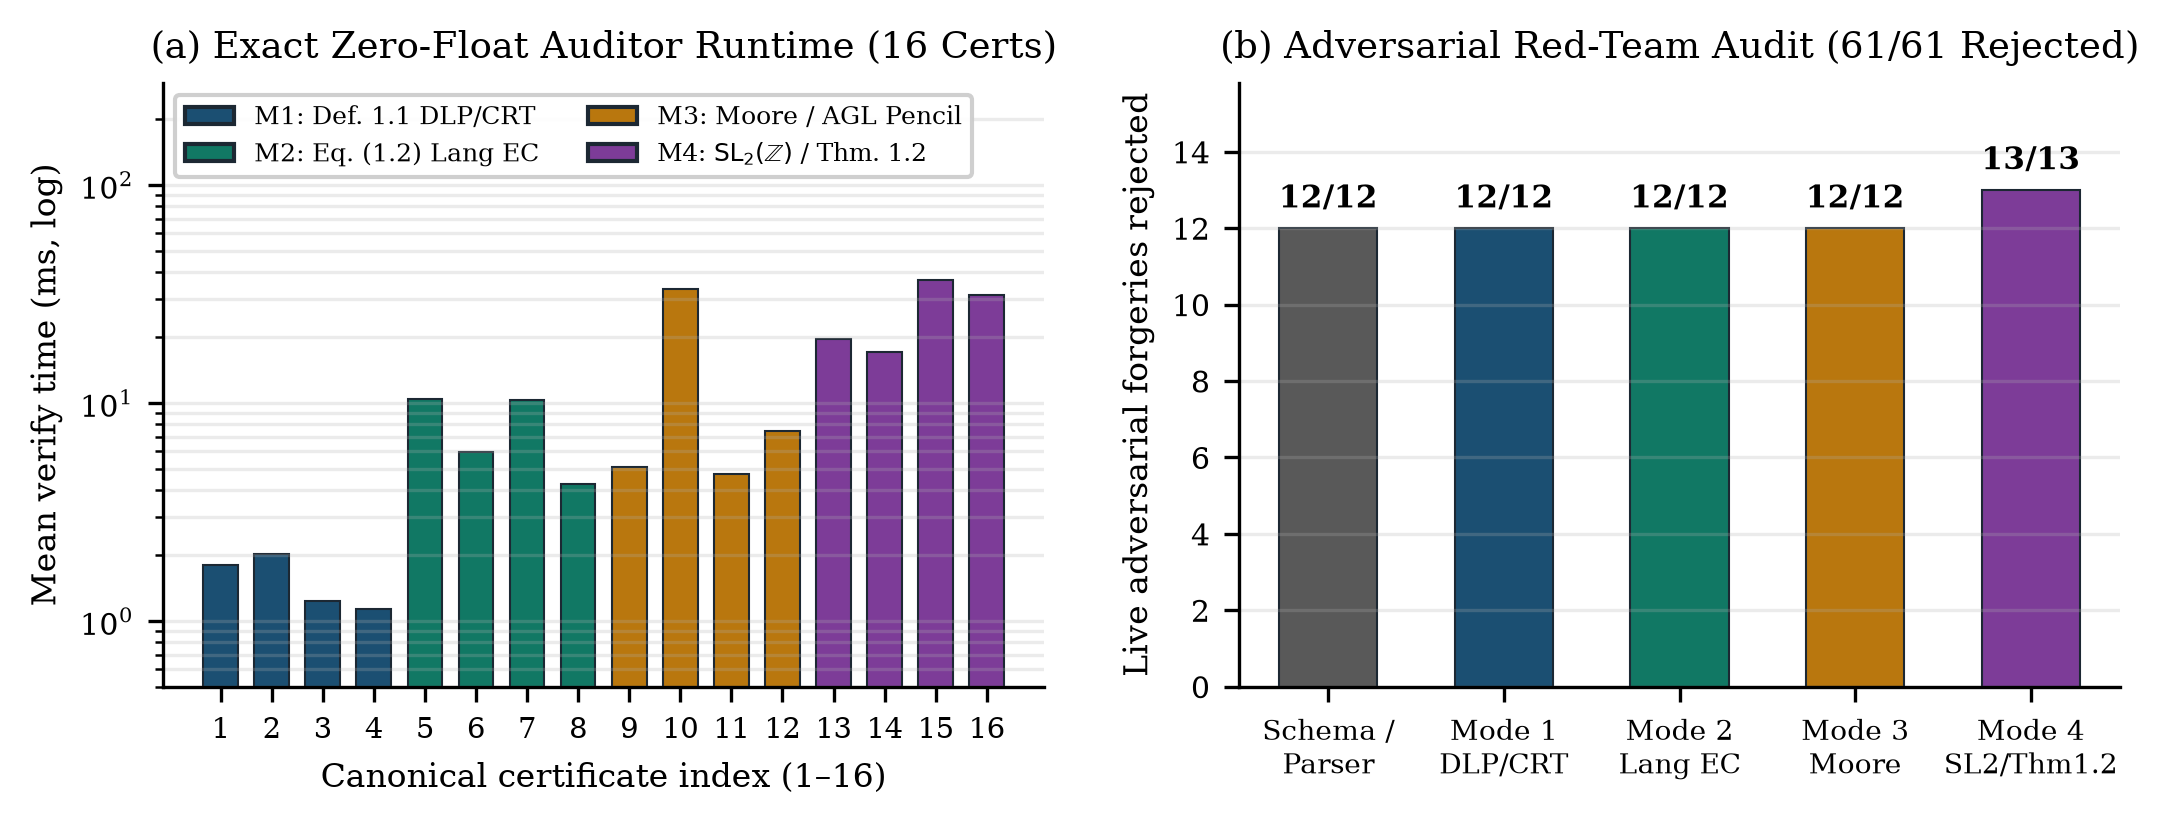
\includegraphics[width=\columnwidth]{figures/fig3_atlas_and_redteam.png}
\vspace{-1.3em}
\caption{\textbf{(a)}~Mean exact zero-float verification latency across all 16 canonical certificates ($1.133$--$36.640\,\mathrm{ms}$, log scale). \textbf{(b)}~Live adversarial red-team audit rejecting 61/61 forgeries across five attack classes with exact error-branch assertions.}
\label{fig:atlas}
\end{figure}

\paragraph{3. 16-Certificate Atlas \& 65-Test Red-Team Audit (Table~\ref{tab:atlas}, Fig.~\ref{fig:atlas}).}
Table~\ref{tab:atlas} lists all 16 canonical certificates verified in $1.133$--$36.640\,\mathrm{ms}$. \nolinkurl{tests/test_suite.py} executes 65 pytest functions: 1 aggregate replay of all 16 certificates, 3 raw-JSON parser checks (IEEE-754 float, \texttt{NaN}, duplicate keys), and 61 parametrized live adversarial forgery tests (12 schema/parser + 12 each for Modes~1--3 + 13 for Mode~4, including supersingular curve forgery, Lang-sign negation $\phi_q(-I_0)\ne -I_0+Q$, all four Lemma~3.3 (A1)--(A4) breaks, trivial $\gamma=1$ base forgery, rank-deficient composite relation matrices, and $\ell_2=25{,}087$ sub-threshold $B=3$), each asserting an exact regex match on the expected rejection branch. \nolinkurl{scripts/verify_all.py} enforces all 5 gates including strict axiom whitelisting and a 41-file SHA-256 manifest.

\begin{table}[t]
\centering
\caption{Canonical 16-certificate \nolinkurl{DLP-COGENTIC-CERT-1.0} atlas (\nolinkurl{results/exp1_certificate_atlas.json}; all 16 verified).}
\label{tab:atlas}
\scriptsize
\setlength{\tabcolsep}{2.2pt}
\resizebox{\columnwidth}{!}{%
\begin{tabular}{@{}l c l r@{}}
\toprule
Certificate ID & M & Exact Certified Witness Summary & ms \\
\midrule
\texttt{m1\_dlp\_f2\_16\_log\_crt} & M1 & $\FF_{2^{16}}^\times$: \texttt{LOG} $x{=}41927$, CRT $15{\cdot}4369$ & 1.815 \\
\texttt{m1\_dlp\_f3\_12\_log\_crt} & M1 & $\FF_{3^{12}}^\times$: \texttt{LOG} $x{=}314159$, CRT $80{\cdot}6643$ & 2.022 \\
\texttt{m1\_dlp\_f2\_20\_not\_in\_subgroup} & M1 & $\FF_{2^{20}}^\times$: \texttt{NOT\_IN\_SUBGROUP} $E{=}209715$ & 1.231 \\
\texttt{m1\_dlp\_f5\_10\_not\_in\_subgroup} & M1 & $\FF_{5^{10}}^\times$: \texttt{NOT\_IN\_SUBGROUP} $E{=}887784$ & 1.133 \\
\texttt{m2\_lang\_p2\_f16\_order5} & M2 & $p{=}2, q{=}16$: $N_E{=}20, t{=}-3$, Eq.~\eqref{eq:lang} ok & 10.417 \\
\texttt{m2\_lang\_p3\_f9\_order5} & M2 & $p{=}3, q{=}9$: $N_E{=}15, t{=}-5$, Eq.~\eqref{eq:lang} ok & 5.946 \\
\texttt{m2\_lang\_p5\_f25\_order5} & M2 & $p{=}5, q{=}25$: $N_E{=}35, t{=}-9$, Eq.~\eqref{eq:lang} ok & 10.330 \\
\texttt{m2\_lang\_p7\_f7\_order5} & M2 & $p{=}7, q{=}7$: $N_E{=}5, t{=}3$, Eq.~\eqref{eq:lang} ok & 4.253 \\
\texttt{m3\_pencil\_p2\_q0\_4\_N2} & M3 & $q_0{=}4,q{=}64,N{=}2$: $|\mathrm{AGL}|{=}2880$, 16 rts & 5.111 \\
\texttt{m3\_pencil\_p2\_q0\_4\_N3} & M3 & $q_0{=}4,q{=}256,N{=}3$: $|\mathrm{AGL}|{=}1.16{\cdot}10^7$, 64 rts & 33.177 \\
\texttt{m3\_pencil\_p3\_q0\_3\_N2} & M3 & $q_0{=}3,q{=}81,N{=}2$: $|\mathrm{AGL}|{=}432$, 9 rts & 4.730 \\
\texttt{m3\_pencil\_p5\_q0\_5\_N2} & M3 & $q_0{=}5,q{=}125,N{=}2$: $|\mathrm{AGL}|{=}12000$, 25 rts & 7.430 \\
\texttt{m4\_unimodular\_f2\_16\_composite\_log} & M4 & $M_L{=}4369$: \texttt{LOG}, $K{=}4,R{=}8$, $B{=}4$ & 19.666 \\
\texttt{m4\_unimodular\_f3\_12\_composite\_nonmem} & M4 & $M_L{=}6643$: \texttt{NONMEM}, $K{=}4,R{=}8$, $B{=}5$ & 17.052 \\
\texttt{m4\_unimodular\_f2\_20\_composite\_log} & M4 & $M_L{=}13981$: \texttt{LOG}, $K{=}5,R{=}10$, $B{=}7$ & 36.640 \\
\texttt{m4\_unimodular\_f5\_10\_composite\_nonmem} & M4 & $M_L{=}406901$: \texttt{NONMEM}, $K{=}5,R{=}10$, $B{=}14$ & 31.176 \\
\bottomrule
\end{tabular}}
\end{table}

\section{Conclusion}\label{sec:conc}
We delivered an independent, explicitly scoped, zero-floating-point verification stack for Google Research Cogentic's sub-quasi-polynomial Discrete Logarithm breakthrough~\cite{cogentic2026dlp}, pairing 18 constructive Lean~4.35.0 theorems (zero \texttt{sorry}, zero \texttt{Classical.choice}) with the pure-\texttt{int} auditor \nolinkurl{DLP-COGENTIC-CERT-1.0}, 16 canonical exact witnesses spanning all characteristics $p\in\{2,3,5,7\}$, exact Theorem~1.2(2) onset characterization ($\ell_2=25{,}088$), and 61/61 live adversarial forgery rejections.

{\footnotesize
\bibliographystyle{plain}
\bibliography{references}}
\end{document}
